
\de{ĐỀ THI HỌC KỲ I NĂM HỌC 2022-2023}{THPT Trần Quang Khải}



\begin{bt}%[0T1B3-1]%[0T1B3-2]%[Dự án đề kiểm tra HK1 22-23-Nhật Thiện]%[Trường TRẦN QUANG KHẢI]
\begin{listEX}
\item Cho tập hợp $A=\left\{x \in \mathbb{R}\mid x^2-5 x-6=0\right\}$; $B=\{1 ;-1\}$. Xác định tập hợp $A \setminus B$.
\item Biết $D=\{x \in \mathbb{R}\mid 1 \leq x \leq 5\}$; $E=\{x \in \mathbb{R}\mid 3<x \leq 6\}$. Tìm $D \cap E$ và $D \cup E$.
\end{listEX}
\loigiai{
	\begin{listEX}
		\item Ta  có $x^2-5x-6=0\Leftrightarrow \hoac{&x=-1\\&x=6.}$\\
		Suy ra $A=\{-1;6\}$.\\
		Vậy  $A \setminus B=\{6\}$.
		\item Ta có $D=[1;5]$, $E=(3;6]$.\\
		Suy ra $D \cap E=(3;5]$; $D \cup E=[1;6]$.
	\end{listEX}
}
\end{bt}

\begin{bt}%[0T3B1-2]%[Dự án đề kiểm tra HK1 22-23-Nhật Thiện]%[Trường TRẦN QUANG KHẢI]
	Tìm tập xác định của các hàm số sau
\begin{listEX}[2]
\item $y=f(x)=\dfrac{8 x+3}{x^2-4}$;
\item $y=g(x)=\dfrac{1}{\sqrt{6-3x}}$.
\end{listEX}
\loigiai{
	\begin{listEX}
		\item Điều kiện xác định của hàm số là $x^2-4\ne 0\Leftrightarrow \heva{&x\ne 2\\&x\ne -2.}$\\
		Vậy tập xác định của hàm số là $\mathscr{D}=\mathbb{R}\setminus\{2;-2\}$.
		\item Điều kiện xác định của hàm số là $6-3x>0\Leftrightarrow x<2$.\\
		Vậy tập xác định của hàm số là $\mathscr{D}=(-\infty;2)$.
	\end{listEX}
}
\end{bt}

\begin{bt}%[0T3B2-2]%[Dự án đề kiểm tra HK1 22-23-Nhật Thiện]%[Trường TRẦN QUANG KHẢI]
Cho hàm số bậc hai $y=f(x)=ax^2+bx+c$ có $f(0)=1$, $f(1)=-4$, $f(2)=-7$. Hãy xác định giá trị của các hệ số $a$, $b$ và $c$.
\loigiai{
	Ta có $\heva{&f(0)=1\\&f(1)=-4\\&f(2)=-7}\Leftrightarrow \heva{&c=1\\&a+b+c=-4\\&4a+2b+c=-7}\Leftrightarrow \hoac{&a=1\\&b=-6&c=1.}$
}
\end{bt}

\begin{bt}%[0T3B2-1]%[Dự án đề kiểm tra HK1 22-23-Nhật Thiện]%[Trường TRẦN QUANG KHẢI]
	Cho hàm số bậc hai $y=-x^2+2 x+m$. Hãy xác định giá trị của $m$ để hàm số đạt giá trị lớn nhất bằng $5$.
\loigiai{
Đỉnh $S$ của parabol có tọa độ $x_S=-\dfrac{b}{2a}=-\dfrac{2}{2\cdot (-1)}=1$; $y_S=-1^2+2\cdot 1+m=m+1$.\\
Hàm số đạt giá trị lớn nhất bằng $5$ khi $y_S=5\Leftrightarrow m+1=5\Leftrightarrow m=4$ tại $x_S=2$.
}
\end{bt}

\begin{bt}%[0T5B2-5]%[0T5B4-1]%[Dự án đề kiểm tra HK1 22-23-Nhật Thiện]%[Trường TRẦN QUANG KHẢI] 
Cho hình vuông $ABCD$ có cạnh bằng $4$.
\begin{listEX}[2]
\item Tính độ dài của véc-tơ $\vec{a}=\vec{AB}+\vec{AD}$
\item Tính tích vô hướng $\vec{BA}\cdot \vec{BC}$.
\end{listEX}
\loigiai{
\begin{listEX}
	\item Ta có $\vec{a}=\vec{AB}+\vec{AD}=\vec{AC}$.\\
	Suy ra độ dài véc-tơ $\vec{a}$ bằng $AC=AB\sqrt{2}=4\sqrt{2}$.
	\item Ta có $\vec{BA}\cdot \vec{BC}=BA\cdot BC\cdot \cos \widehat{ABC}=\cdot 4\cdot 4\cos 45^\circ=8\sqrt{2}$.
\end{listEX}
}
\end{bt}

\begin{bt}%[0T5B3-4]%[Dự án đề kiểm tra HKII NH22-23 - Thy Nguyen Vo Diem]%[THPT Trần Quang Khải]
Cho tứ giác $ABCD$. Gọi $M$ và $N$ lần lượt là trung điểm các cạnh $AB$ và $CD$.
\begin{listEX}
\item Chứng minh rằng $\vec{AC}+\vec{BD}=2\vec{MN}$.
\item Gọi $K$ là điểm trên cạnh $AC$ sao cho $AK=\dfrac{2}{3}AC$, $I$ là trung điểm của $MK$.\\
Chứng minh rằng $\vec{AI}=\dfrac{1}{4}\vec{AB}+\dfrac{1}{3}\vec{AC}$.
\end{listEX}
\loigiai{
\begin{listEX}
	\item $M$ là trung điểm các cạnh $AB$ nên $\vec{MA}+\vec{MB}=\vec{0} \Leftrightarrow \vec{AM}+\vec{BM}=\vec{0}$.\\
	$N$ là trung điểm các cạnh $CD$ nên $\vec{NC}+\vec{ND}=\vec{0}$.\\
	Do đó \allowdisplaybreaks{\begin{eqnarray*}
		\vec{AC}+\vec{BD}	&=& \left(\vec{AM}+\vec{MN}+\vec{NC}\right)+\left(\vec{BM}+\vec{MN}+\vec{ND} \right)\\
			&=& \left(\vec{AM}+ \vec{BM}\right)+2\vec{MN}+\left( \vec{NC}+ \vec{ND}\right) \\
			&=& 2\vec{MN}.
	\end{eqnarray*}}
	\item \immini{$I$ là trung điểm của $MK$ nên \allowdisplaybreaks{\begin{eqnarray*}
		\vec{AI}	&=& \dfrac{1}{2}\left(\vec{AM}+\vec{AK}\right) \\
			&=& \dfrac{1}{2}\cdot \dfrac{1}{2}\vec{AB}+\dfrac{1}{2}\cdot \dfrac{2}{3}\vec{AC} \\
			&=&  \dfrac{1}{4}\vec{AB}+\dfrac{1}{3}\vec{AC}.
	\end{eqnarray*}}
}
{
	\begin{tikzpicture}[>=stealth,scale=1, line join = round, line cap = round]
	\path (-2,0) coordinate (D)
	(3,0) coordinate (C)
	(2.5,2.5) coordinate (B)
	(-1,3) coordinate (A)
	($(A)!1/2!(B)$) coordinate (M)
	($(C)!1/2!(D)$) coordinate (N)
	($(A)!2/3!(C)$) coordinate (K)
	($(K)!1/2!(M)$) coordinate (I)
	;
	\draw (A)--(B)--(C)--(D)--(A) (A)--(C) (M)--(K) (A)--(I);
	\foreach \x/\goc in {A/90,B/60,C/0,D/180,N/-90,M/90,K/60,I/0}\fill[black]
	(\x) circle (1pt)
	($(\x)+(\goc:3mm)$)node{$\x$};
\end{tikzpicture}
}
\end{listEX}
}
\end{bt}


\begin{bt}%[0T5B4-7]%[Dự án đề kiểm tra HKII NH22-23 - Thy Nguyen Vo Diem]%[THPT Trần Quang Khải]
Một người dùng một lực $\vec{F}$ có độ lớn $100 $N để kéo một thùng hàng dịch chuyển một đoạn $15$m. Biết lực $\vec{F}$ hợp với hướng dịch chuyển một góc $60^{\circ}$. Tính công sinh bởi lực $\vec{F}$.
\loigiai{
\immini{Công sinh bởi lực $\vec{F}$ là $$\left|\vec{F}\right| \left|\vec{d} \right|\cos \left(\vec{F},\vec{d}\right)=100 \cdot 15 \cdot \cos 60^\circ=750 \ (\mathrm{N}).$$}{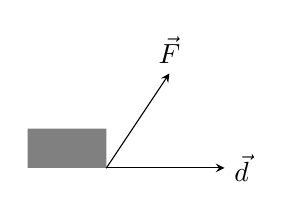
\begin{tikzpicture}[>=stealth,scale=1, line join = round, line cap = round]
	\fill[gray] (0,0)--(0,0.5)--(1,0.5)--(1,0)--(0,0);
	\draw[->] (1,0)--(2.5,0) node[right]{$\vec{d}$};
	 \draw[->] (1,0)--(1.8,1.2) node[above]{$\vec{F}$};
\end{tikzpicture}
}
}
\end{bt}


\begin{bt}%[0T6B3-4]%[Dự án đề kiểm tra HKII NH22-23 - Thy Nguyen Vo Diem]%[THPT Trần Quang Khải]
Xoài cát Hòa Lộc là loại xoài đặc sản nổi tiếng của vùng đồng bẳng sông Cửu Long. Một năm xoài có hai mùa, mùa thuận là từ tháng 3 đến tháng 5, mùa nghịch là từ tháng 10 đến tháng 12. Xoài có thể ra trái sau 24 tháng trồng. Năm 2005, Cục Sở hữu trí tuệ thuộc Bộ Khoa học và Công nghệ cấp văn bằng bảo hộ độc quyền nhãn hiệu tập thể cho sản phẩm Xoài cát Hòa Lộc. Xoài cát Hòa Lộc được xuất khẩu sang các nước Pháp, Mỹ, Canada\ldots\\
Bạn Hoa chọn ngẫu nhiên 10 trái xoài cát Hòa Lộc và ghi lại khối lượng ở bảng sau (đơn vị: gam).
\begin{center}
\begin{tabular}{|l|l|l|l|l|l|l|l|l|l|}
\hline 450 & 510 & 510 & 600 & 480 & 420 & 510 & 450 & 650 & 540 \\
\hline
\end{tabular}
\end{center}
\begin{listEX}
\item Em hãy tính khối lượng trung bình $\overline{x}$ của một trái xoài ở bảng trên. Nếu bạn Hoa muốn mua $3 $ kg xoài thì sẽ được khoảng bao nhiêu trái?
\item Em hãy tìm mốt $M_o$ của khối lượng xoài ở mẫu số liệu trên.
\end{listEX}
\loigiai{
\begin{listEX}
	\item Khối lượng trung bình $\overline{x}$ của một trái xoài là $$\overline{x}=\dfrac{450\cdot 2+510\cdot 3+600+480+420+650+540}{10}=512 \ (\text{gam}).$$
	Hoa muốn mua 3 kg xoài thì sẽ được $\dfrac{3}{0{,}512}=5{,}8 \approx 6$ trái.
	\item Mốt $M_o$ của khối lượng xoài ở mẫu số liệu trên là $510$ vì tần số của $510$ là $3$ lớn nhất trong mẫu số liệu.
\end{listEX}
}
\end{bt}
\begin{bt}%[0T2B1-3]%[Dự án đề kiểm tra HKII NH22-23 - Thy Nguyen Vo Diem]%[THPT Trần Quang Khải]
	Một học sinh dự định vẽ các tấm thiệp xuân làm bằng tay để bán trong hội chợ Tết. Cần $ 2 $ giờ để vẽ tấm thiệp loại nhỏ có giá $ 10 $ nghìn đồng và 3 giờ để vẽ tấm thiệp loại lớn có giá 20 nghìn đồng. Học sinh này chỉ có 30 giờ để vẽ và ban tổ chức hội chợ yêu cầu phải vẽ ít nhất 12 tấm. Hãy cho biết bạn ấy phải vẽ bao nhiêu tấm thiệp mỗi loại để có nhiều tiền nhất?
\loigiai{
\immini{Gọi $x$ và $y$ lần lượt là số thiệp loại nhỏ và loại lớn.\\
Ta có hệ bất phương trình sau
\[\heva{& x+y \geq 12 \\ & 2x+3y \leq 30 \\ & x \geq 0 \\ & y \geq 0.}\]	
Biểu diễn miền nghiệm của hệ bất phương trình ta được miền tam giác $ABC$ có toạ độ các đỉnh là $A(12;0)$, $B(15;0)$, $C(6;6)$.\\
Số tiền bạn đó thu được $F=10x+20y$ đạt giá trị lớn nhất là 180 nghìn đồng tại đỉnh $C(6;6)$.
}{
\begin{tikzpicture}[scale=1, font=\footnotesize, line join=round, line cap=round, >=stealth]
	\draw[->] (-1,0)--(6,0) node[above]{$x$};
	\draw[->] (0,-1)--(0,5) node[right]{$y$};
	\draw[fill=black] (0,0) circle (1pt) node[below left] {$O$};
	\draw[fill=black] (0,4) circle (1pt) node[left]{$12$};
	\draw[fill=black] (0,10/3) circle (1pt) node[left]{$10$};
	\draw[fill=black] (5,0) circle (1pt) node[below]{$15$};
	\draw[fill=black] (4,0) circle (1pt) node[below left]{$12$};
	\draw[fill=black] (2,2) circle (1pt);
	\draw [domain=-1:4.7, samples=100] plot (\x, {-\x+4});
	\draw [domain=-1:6, samples=100] plot (\x, {-2/3*\x+10/3});
	\tkzDefPoints{4/0/A,5/0/B,2/2/C}
	\tkzDrawPolygon[fill=gray,opacity=.2](A,B,C)
	\tkzLabelPoints[above left=-0.1 and 0.2](A)
	\tkzLabelPoints[above right=-0.1 and 0](B)
	\tkzLabelPoints[above right](C)
\end{tikzpicture}
}
}
\end{bt}